\documentclass[11pt,a4paper]{article}
\usepackage[margin=25mm,headheight=14pt]{geometry}
\usepackage[T1]{fontenc}
\usepackage{lmodern}
\usepackage{microtype}
\usepackage{graphicx}
\usepackage{booktabs,tabularx,longtable,array}
\usepackage{amsmath}
\usepackage{xcolor}
\usepackage{fancyhdr}
\usepackage{caption}
\usepackage[hidelinks]{hyperref}
\usepackage{enumitem}
\definecolor{navy}{HTML}{15334A}
\definecolor{teal}{HTML}{176B87}
\captionsetup{font=small,labelfont=bf}
\setlength{\parskip}{5pt}
\setlength{\parindent}{0pt}
\setlist{nosep,leftmargin=1.5em}
\pagestyle{fancy}\fancyhf{}
\fancyhead[L]{\small ExpiryWatch India}\fancyhead[R]{\small Work Package 5}
\fancyfoot[C]{\thepage}
\newcommand{\banner}{\begin{center}\colorbox{navy}{\parbox{0.94\linewidth}{\centering\color{white}\textbf{SURVEILLANCE PRIORITY ONLY -- NOT EVIDENCE OF MANIPULATION}}}\end{center}}
\newcommand{\bps}{\,\mathrm{bp}}
\begin{document}
\begin{titlepage}\centering\vspace*{22mm}
{\Large ExpiryWatch India\par}\vspace{18mm}
{\color{navy}\Huge\bfseries Work Package 5\par}\vspace{8mm}
{\Large Cross-Market Price-Influence Diagnostics -- Spot-Only Subset\par}\vspace{18mm}
\rule{0.72\linewidth}{0.7pt}\par\vspace{12mm}
{\large Alhat Ayush Arvind (24110028)\par}\vspace{4mm}
{\large NIFTY 50 spot-only empirical prototype\par}\vfill
{\large 18 November 2026\par}\vspace{5mm}
{\small Work-package report; results based on the supplied project outputs}\par
\end{titlepage}
\banner
\begin{abstract}
This report evaluates the WP5 diagnostics that can be estimated from two-hour NIFTY spot data and matched controls. Across 367 S1 expiries, elevated final-bar activity is concentrated in monthly expiries and the 2023--2026 era, while strike proximity, next-day reversal and serial recurrence provide limited or non-robust evidence. Constituent concentration, price impact and cross-market asymmetry remain unmeasured because the required constituent, flow, options and futures data are absent. The findings describe market behaviour and surveillance priority only.
\end{abstract}
\tableofcontents\clearpage
\section{Purpose and scope}
Work Package 5 in the project proposal asks whether expiry-related price movement is concentrated in settlement-relevant time, a small set of index constituents, low-flow/high-impact episodes, or derivative-linked cross-market patterns. This report documents the subset that can be computed from NIFTY spot prices at two-hour frequency and the existing matched-control workbook. The data support the final 15-minute bar and next-day diagnostics, plus an unweighted close-to-strike check. They do not support a full cross-market price-influence analysis.

All scores and elevated observations are research screening outputs. They do not identify actors, intent, or a legal violation. The CAS period is excluded: the input has nine CAS expiries and the Step 2/3/4 package is restricted to comparable S1 sessions.

\section{Inputs and sample}
The analysis uses the NIFTY spot series and WP1/WP2 workbook in the project data directory, the five WP5 result tables in the results package, and the matching logic already implemented in WP2. The analysis sample contains 367 S1 expiries with three matched controls each: 282 weekly and 85 monthly. Four otherwise eligible expiries are omitted after feature warm-up; nine CAS expiries are outside this S1 sample. The settlement-relevant interval observable in the supplied bar structure is 15:15--15:30 only. Controls are drawn within plus or minus 60 calendar days; the matching and standardisation inherit the WP2 full-sample design and therefore have mild look-ahead exposure.

\section{Methods}
\subsection{Settlement timing}
For each expiry, final-bar absolute return, final-bar high-low range, and the final bar's share of the four-bar daily price path are compared with the mean of three matched non-expiry controls. The primary contrast is the expiry-minus-control difference. The tables report Welch tests, Wilcoxon tests, and Benjamini--Hochberg adjusted q-values within each result table. Results are also grouped by expiry type and broad era (2019--2022 and 2023--2026). These are subgroup descriptions, not a causal reform design.

\subsection{Concentration, strike alignment, reversal and recurrence}
Effect concentration sorts expiry-minus-control differences and reports how much positive excess is carried by the largest 5, 10 and 20 percent of events. Strike distance is computed from the 15:30 spot close, on 50- and 100-point grids, without open-interest weighting; under a uniform fractional strike position, the expected mean fractional distance is 0.25 and the expected share within 0.05 is 10 percent. Next-day reversal is the signed next-day return difference relative to controls, with positive values defined as movement against the expiry-day direction. Recurrence is assessed using lag-one autocorrelation and permutation tests of consecutive same-type top-decile events; pair-test q-values use BH correction.

\section{Results}
\subsection{Settlement-window activity}
Across all 367 expiries, final-15-minute absolute return is 1.48 basis points higher than controls (19.2 percent relative; Welch $p=0.004$, BH $q=0.009$). Final-bar range is 1.88 basis points higher (12.0 percent; $p<0.001$, $q<0.001$), and the final-bar share of the daily path is 2.03 percentage points higher ($p<0.001$, $q=0.002$). The effect differs by expiry type: weekly absolute return is 0.53 basis points higher (6.9 percent; $p=0.328$), whereas monthly absolute return is 4.62 basis points higher (60.4 percent; $p<0.001$). Monthly final-bar range is 6.91 basis points higher (44.7 percent; $p<0.001$). The weekly estimates are small and not statistically distinguishable from zero in this comparison.

The broad era split is also marked. For 2019--2022 the absolute-return difference is -0.13 basis points ($p=0.865$); for 2023--2026 it is +3.02 basis points, or 49.5 percent ($p<0.001$, BH $q<0.001$). The later-era estimate is descriptive and overlaps changes in expiry composition and market rules; it is not an estimate of the effect of a specific policy.

\begin{figure}[htbp]\centering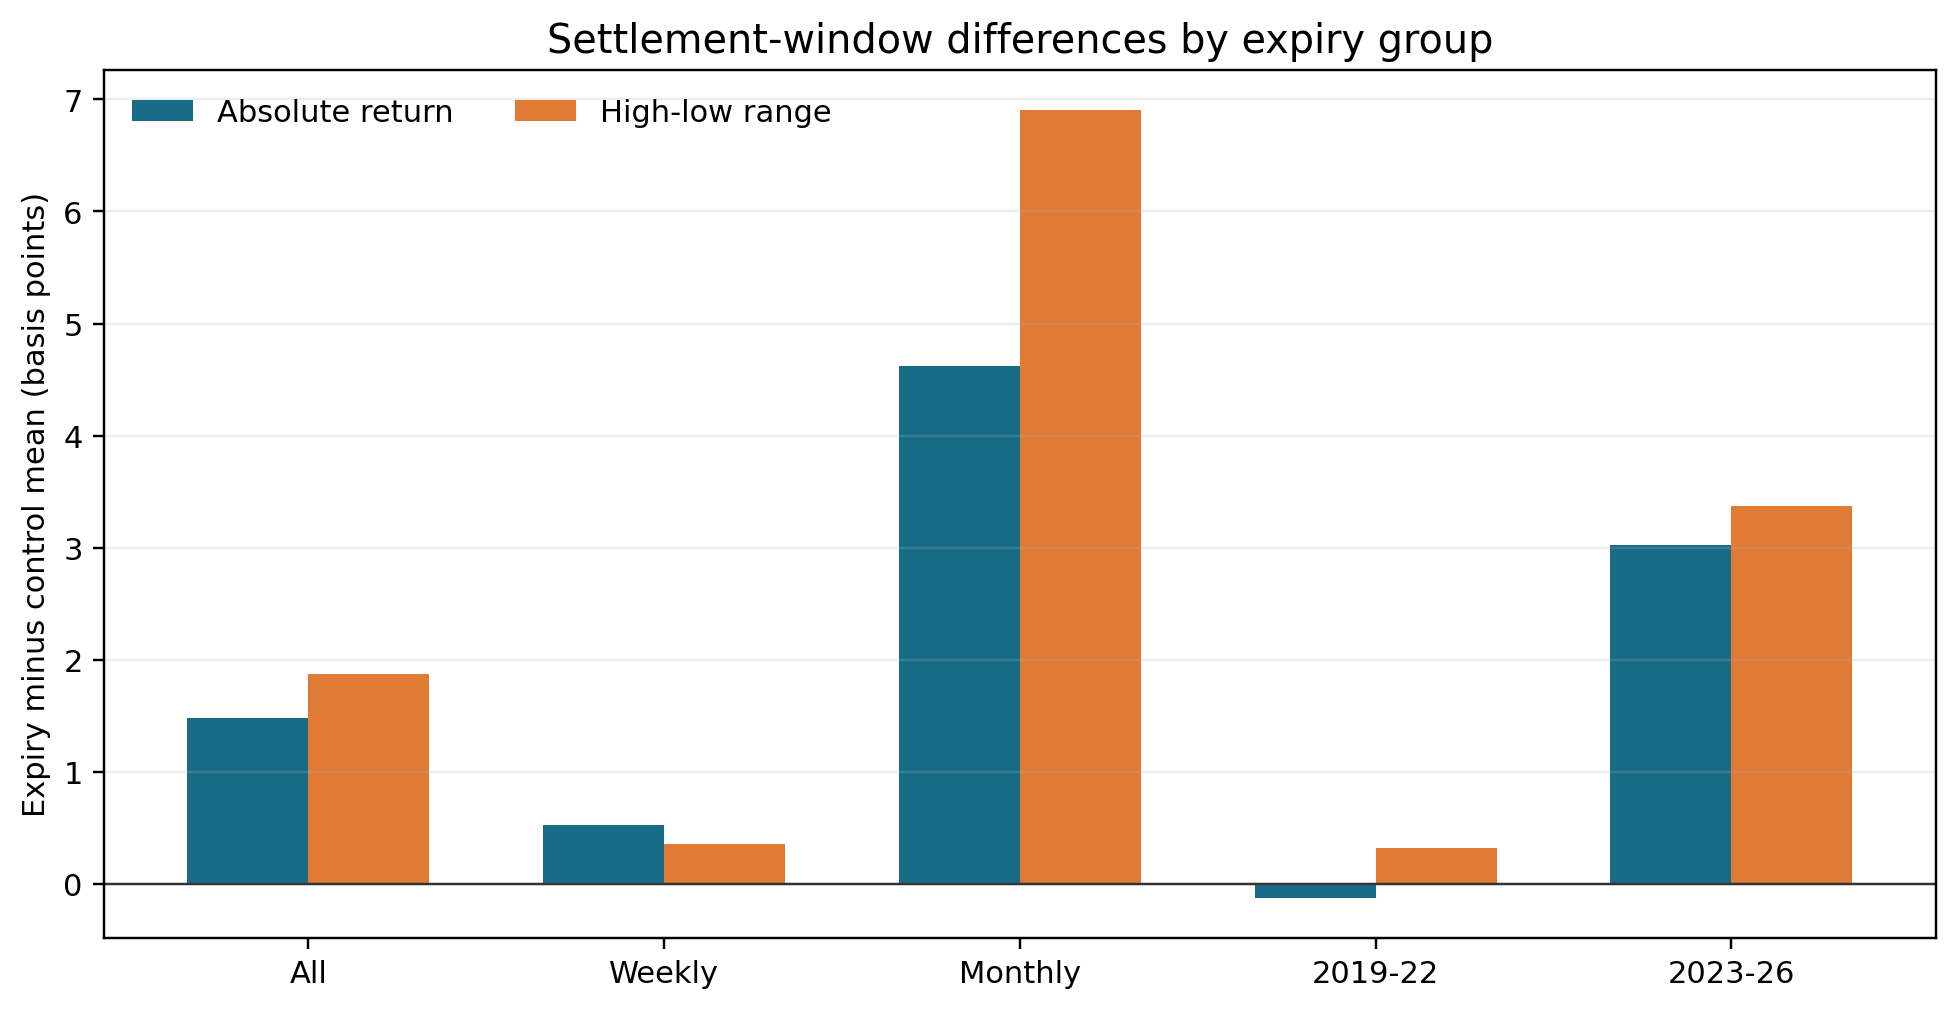
\includegraphics[width=0.92\linewidth]{wp5_settlement_differences.png}\caption{Expiry-minus-control means for final-bar absolute return and range. Values are in basis points; era groups overlap with expiry-type composition.}\end{figure}

\begin{table}[htbp]\centering\caption{Table 1: Primary settlement-timing contrasts}\small
\begin{tabular}{lrrrr}\toprule Group & $n$ & $|r_4|$ diff. (bp) & Relative & Range diff. (bp)\\\midrule
All S1 expiries & 367 & +1.48 & +19.2\% & +1.88\\
Weekly & 282 & +0.53 & +6.9\% & +0.36\\
Monthly & 85 & +4.62 & +60.4\% & +6.91\\
2019--2022 & 180 & -0.13 & -1.3\% & +0.32\\
2023--2026 & 187 & +3.02 & +49.5\% & +3.37\\\bottomrule\end{tabular}
\caption*{Welch two-sided $p$ for all / weekly / monthly / 2019--22 / 2023--26 absolute-return contrasts: 0.004 / 0.328 / $<0.001$ / 0.865 / $<0.001$.}
\end{table}

\subsection{Concentration and strike alignment}
The top 10 percent of expiries (37 events) account for 52.6 percent of the total positive excess final-bar absolute return and 150.5 percent of net excess. A share above 100 percent means the remaining events net to a negative contribution. This concentration describes the distribution of the measured timing effect; it is not constituent-level influence concentration.

Across the full sample, mean distance to the nearest 50-point grid is 0.244 (uniform-position reference 0.250); 11.4 percent of closes fall within 0.05 of a 50-point strike compared with 10 percent expected ($p=0.339$, BH $q=0.678$). The corresponding 100-point share is 8.2 percent ($p=0.296$). Monthly 100-point proximity is 3.5 percent ($p=0.045$), but does not survive the within-table correction ($q=0.454$). The evidence does not support a robust spot-close pinning result. These distances are not open-interest-weighted and the close is not the settlement VWAP.

\subsection{Reversal and recurrence}
Mean next-day signed reversal difference is +0.115 percentage points for all expiries ($p=0.090$, BH $q=0.383); weekly is +0.076 points ($q=0.383) and monthly +0.245 points ($q=0.383). None of the reported conditional groups survives correction. The pattern is therefore weak evidence of reversal, not a reliable post-expiry reversal effect.

No lag-one autocorrelation is significant after correction for either weekly or monthly expiries. One nominal recurrence result appears for weekly last-bar-share differences: seven consecutive top-decile pairs versus 2.84 expected under random ordering ($p=0.014$), but BH $q=0.086$. It does not pass the stated 5 percent corrected threshold. Quarter-end monthly comparisons are also non-significant (final-bar absolute return $p=0.833$; range $p=0.578$; last-bar share $p=0.981$). The annual share of type-specific top-decile events varies from 4 to 17 percent, without a systematic pattern established by this descriptive summary.

\section{WP5 coverage and unmet requirements}
\begin{table}[htbp]\centering\caption{Table 2: Proposal diagnostics and data status}\small
\begin{tabularx}{\linewidth}{p{0.24\linewidth}p{0.18\linewidth}X X}\toprule Diagnostic & Status & Limitation in this run & Data required\\\midrule
Settlement timing concentration & Partial & Final 15 minutes only; final hour/30/5 minutes and settlement VWAP are unavailable & Minute-level index prices and settlement prints\\
Index-contribution concentration (WPPI/EIC) & Not built & No component returns or weights in the analysis input & Historical NIFTY constituent prices and index weights\\
Price impact (Kyle $\lambda$) & Not built & No signed flow, turnover, or order-book depth & Trade/order data with direction and volume\\
Cross-market asymmetry (CMBR) & Not built & No option/futures exposure or participant positioning & F\&O bhavcopy, options OI by strike, futures basis; participant data for expanded test\\
Strike/payoff alignment & Partial & Spot close, equally weighted; no option OI weighting & F\&O bhavcopy with strike-level OI and settlement values\\
Reversal & Partial & Next trading day only; news and intraday dynamics are not controlled & Intraday post-expiry data and WP7 event/news retrieval\\
Recurrence & Partial & NIFTY only; same-type event sequence & Comparable BANKNIFTY, FINNIFTY and SENSEX expiry series\\\bottomrule\end{tabularx}\end{table}

\section{Limitations and interpretation}
The two-hour bar source resolves the last 15 minutes from the 15:15 bar but cannot reconstruct finer settlement windows. Matched controls are observational and can differ in unmeasured state. The broad era split can reflect policy, lot-size, tax, weekday, and expiry-composition changes; it should not be read causally. P-values are exploratory, and BH correction is performed within each listed table rather than across every analysis in the project. Weekly expiries form a time sequence, so independent-observation tests may overstate precision. Strike analysis omits OI and uses the close. The sample excludes CAS expiries. These results are descriptive market-behaviour diagnostics and cannot establish price influence by any participant.

\section{Implications for later work}
The strongest current finding is a late-session difference concentrated in monthly expiries and the 2023--2026 era, with substantial event-level concentration. The next data step should resolve 5-, 30- and 60-minute windows and combine index moves with constituent contributions, option OI, futures basis, turnover and order-book measures. WP7 should condition selected episodes on dated public information; WP8 should use a separately specified reform design with pre-trend checks and overlapping-rule changes addressed. Until those layers are present, WP5 remains a spot-only subset.

\appendix
\section{Definitions, reproducibility and file map}
Here $r_4$ is the final 15-minute absolute return; range is the high-low range of that bar; last-bar share is its absolute path contribution relative to the four-bar day. The package tables are \texttt{WP5/wp5\_1\_settlement\_timing\_by\_group.csv} through \texttt{wp5\_5\_recurrence\_serial\_dependence.csv}, with supplementary quarter-end and annual tables. The analysis code is \texttt{src/wp5\_wp6\_results.py}; price features and matching are documented in WP1/WP2. Main counts and statistics are in \texttt{RESULTS\_SUMMARY.txt}.

\section{Data dictionary (report variables)}
\begin{description}[style=nextline]
\item[Expiry-minus-control difference] Expiry observation less the mean of its three matched controls.
\item[Final-bar absolute return] Absolute close-to-close return for 15:15--15:30.
\item[Final-bar range] High-low range scaled by the index level.
\item[Last-bar share] Final-bar path measure divided by the four-bar daily path measure.
\item[Fractional strike distance] Distance to the nearest strike grid, divided by grid spacing; zero denotes an exact grid point.
\item[Reversal difference] Next-day signed move against the expiry-day direction, less the matched-control mean.
\item[BH q-value] Benjamini--Hochberg adjusted value within the specified results table.
\end{description}
\end{document}
